\begin{tiny}(Ccu02)\end{tiny}
\begin{figure}[h]
  \centering
  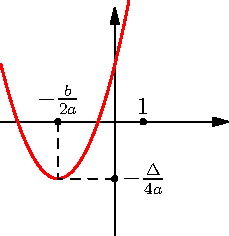
\includegraphics{./Ccu02_1.pdf}
  % Ccu02_1.pdf: 0x0 pixel, 0dpi, 0.00x0.00 cm, bb=
  \caption{Exercice \ref{Ecu02}: Configuration 1.}
  \label{fig:Ccu02_1}
\end{figure}
\begin{enumerate}
  \item On sait que le graphe de la fonction associée à un trinôme est une parabole qui peut être orientée vers le haut ou vers le bas.\newline
  Il convient de détailler (ce qui n'est pas fait ici) dans le cas $a>0$, la preuve de l'équivalence entre l'existence de deux racines $<1$ (Figure \ref{fig:Ccu02_1} : Configuration 1) et les conditions
\begin{displaymath}
  \left\lbrace 
\begin{aligned}
&a>0\\ &-\frac{b}{2a}<1 \\ &\Delta > 0 \\ &a1^2+b1+c >0  
\end{aligned}
\right. 
\end{displaymath}
qui se ramènent facilement à celles de l'énoncé. Le cas $a<0$ est analogue.
  \item On exprime
\begin{align*}
  &a = 2m-1 \\
  &\Delta = -4(m-1)(m+4)\\
  &a+b+c = 5m+4 \\
  &2a+b =6m
\end{align*}
On forme le tableau des signes des expressions à considérer en rangeant les valeurs où le signe change
\begin{displaymath}
  -4  < -\frac{4}{5} < 0 < \frac{1}{2} < 1
\end{displaymath}
On trouve finalement que l'ensemble cherché est
\begin{displaymath}
  [-\frac{5}{4},0[ \,\cup\, ]\frac{1}{2},1[
\end{displaymath}

\end{enumerate}
